%!TEX encoding=UTF-8 Unicode
%!TEX root=../tabarnac.tex

\section{Experimental setup}
\label{sec:metho}

This section briefly discusses our experimental setup for \TABARNAC evaluation
and presents relevant information on the experimental environment.
%presents the hardware architecture, the mapping policies to which we compare
%pour propositions, and the other relevant environment informations.

\begin{table}[htb]
    \centering
    \begin{tabular}{lp{1.1cm}rrp{1.35cm}p{1.1cm}}
        \toprule[.05em]
        %\multirow{3}{.8cm}{CPU}
        %&  & \multicolumn{2}{c}{Vendor} & \multicolumn{2}{c}{Model} \\
        %\cmidrule(lr){3-6}
        \multirow{2}{.8cm}{CPU}& \texttt{Turing}  & \multicolumn{2}{c}{Intel} & \multicolumn{2}{c}{Xeon X7550} \\
        & \texttt{Idfreeze} & \multicolumn{2}{c}{AMD} & \multicolumn{2}{c}{Opteron 6174} \\
        \midrule[.02em]
        \midrule[.02em]
        \multirow{3}{.8cm}{System totals}
        & & Nodes & Threads & Freq & Memory \\
        \cmidrule[.01em](lr){3-6}
        & \texttt{Turing}   & $4$ & $64$ & $2.00$ Ghz & $128$ Gib \\
        & \texttt{Idfreeze} & $8$ & $48$ & $2.20$ Ghz & $256$ Gib\\
        \midrule[.02em]
        \midrule[.02em]
        \multirow{3}{.8cm}{Per node}
        & & Cores & Threads & L3 Cache & Memory \\
        \cmidrule[.01em](lr){3-6}
        & \texttt{Turing}   & $8$ & $16$ & $18$ Mib & $32$ Gib \\
        & \texttt{Idfreeze} & $6$ & $6$  & $12$ Mib & $32$ Gib \\
        \bottomrule[.05em]
    \end{tabular}
    \vspace{4pt}
    \caption{Hardware configuration of our evaluation system.}
    \label{tab:hw}
\end{table}

We used two NUMA machines for our experiments \texttt{Turing} and
\texttt{Idfreeze}. The second machine was only used to compare the
instrumentation overhead on Intel and AMD machines, all the other experiments
ran on \texttt{Turing}. The hardware details are
summarized in Table~\ref{tab:hw}. \texttt{Turing} runs version $3.13$ of the
Linux kernel, while \texttt{Idfreeze} runs version $3.2$.

%\texttt{Turing} is composed of $4$ Intel Xeon X7550
%processors (Nehalem microarchitecture~\cite{Intel2010}). Each processor has its own memory controller and therefore forms a NUMA node. The hardware details are summarized in Table~\ref{tab:Turing}.
%The machine runs version 3.13 of the Linux kernel.
%
%\texttt{Idfreeze} is composed of $4$ AMD Opteron $6174$

%Boths machines are composed of $4$ processors.  Each processor has its own memory
%controller and therefore forms a NUMA node.
%
%\begin{table}[htb]
%    \centering
%    \caption{Hardware configuration of our evaluation system.}
%    \label{tab:Turing}
%    \footnotesize
%        \begin{tabular}{lccccc}
%            \toprule
%            \multirow{2}{1.5cm}{System total} & Nodes & Threads & Freq & Memory \\
%            \cmidrule(lr){2-5}
%                & $4$   & $64$ & $2.00$Ghz & $128$Gib \\
%            \midrule
%            \multirow{2}{1.5cm}{Per NUMA node} & Cores & Threads & L3 Cache & Memory \\
%           \cmidrule(lr){2-5}
%            & $8$ & $16$ & $18$Mib & $32$Gib  \\
%            \bottomrule
%        \end{tabular}
%\end{table}


%\subsection{Applications}

%We evaluate the following applications with \TABARNAC in this paper: %a \emph{matrix multiplication},
%the \emph{IS} benchmark and \emph{Ondes3D}.
%They were chosen to demonstrate different memory access behaviors with different strategies to improve them.

%The \emph{matrix multiplication} is a well-known algorithm that we use to verify the accuracy of \TABARNAC, as well as to discuss the performance improvements that can be achieved.
%The \emph{matrix multiplication} is implemented with Pthreads, while \emph{IS} and \emph{Ondes3D} use OpenMP for parallelization.

All applications use OpenMP for parallelization, they were compiled with
\texttt{gcc}, version 4.6.3, with the \texttt{-O2} optimization flag.  Both
analysis and performance evaluation are performed with $64$ threads,
which is the maximum number of threads that our evaluation machine
(\texttt{Turing}) can execute in parallel.
%The \emph{matrix multiplication} performance was evaluated with
%matrices of size $4096 \times 4096$ doubles and $8192 \times 8192$, resulting on
%a memory usage of $128$Mib and $512Mib$ per matrix.
%\subsection{Mapping Policies}

In the performance evaluation, we compare the following three traditional
mapping policies to the version modified using the knowledge provided by \TABARNAC.
The \emph{original Linux kernel} is our baseline for the experiments. We use an unmodified Linux kernel, version 3.13, with the first-touch policy. The NUMA Balancing mechanism is disabled in this baseline.
The \emph{interleave} policy is performed with the help of the \texttt{numactl} tool.
We also compare our results to the recently introduced \emph{NUMA Balancing} technique~\cite{Corbet}, which is executed with its default configuration.

For the plots presenting speedups, each configuration was executed at least 10 times. Each point represents the arithmetic mean of all runs.
The error bars in those plots represent the standard error.


\section{Analysis and Results}
\label{sec:expe-analysis}

This section presents the results of our analysis.
For each application, we show its memory access behavior, discuss strategies to optimize this behavior and present the performance improvements that can be achieved.

% In this section, we analyze several benchmarks using \TABARNAC, we discuss
% their memory access distribution. Using this analysis we propose some
% optimizations and we evaluate them by comparing it to automatic data mapping
% tools.

% \subsection{Matrix Multiplication}
% \label{sec:exp-mat}

% The first benchmark presented is based on a naive matrix multiplication,
% computing $C=A \times B$. Our aim here is not to provide a kernel competing with the
% state of the art, but to show how \TABARNAC can help to improve such
% applications. We compare two implementations of the matrix multiplication, in
% the first one, called \emph{Naive}, each thread starts by computing
% $C[0][tid]$ and then jumps $N$ elements after in the matrix, where $N$ is the
% number of threads. Although this implementation is known to be inefficient, it is a
% good example of NUMA-unaware code, and comparing the \TABARNAC visualization
% for this algorithm to the one obtained with a better version helps understanding
% how to interpret it.
% Moreover, when an application has such an unstructured memory access pattern, it
% is not always possible to change the pattern completely. Therefore, it is
% interesting to discuss the improvements that can be obtained in this kernel without
% modifying the algorithm.
% The optimized implementation of the matrix multiplication uses a non-recursive block
% decomposition.



% \begin{figure}[htb]
%     \centering
%     \subfigure[Structure B (naive version).]{
%         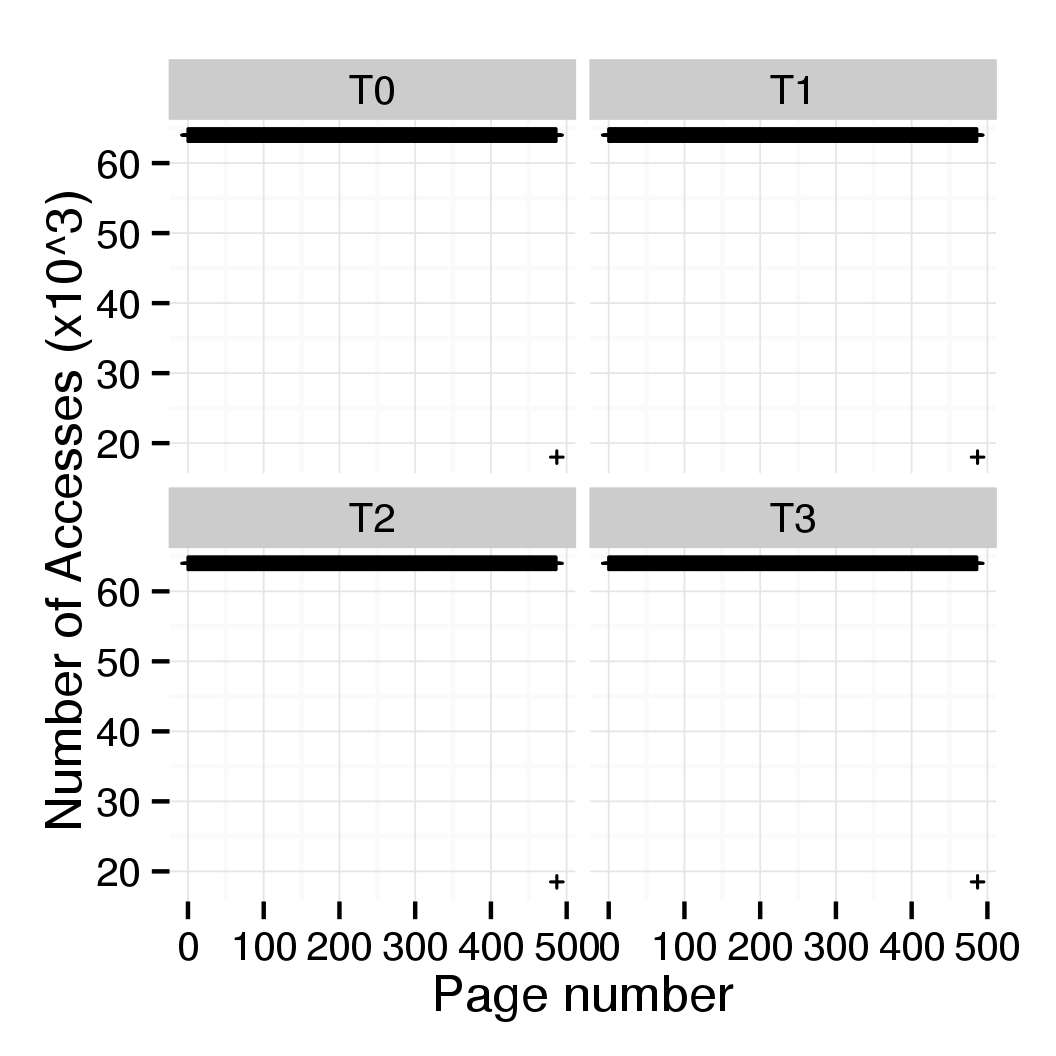
\includegraphics[width=.45\linewidth] {mat_B_modulo}
%         \label{fig:matrix-B-naive}
%     }
%     \subfigure[Structure C (naive version).]{
%         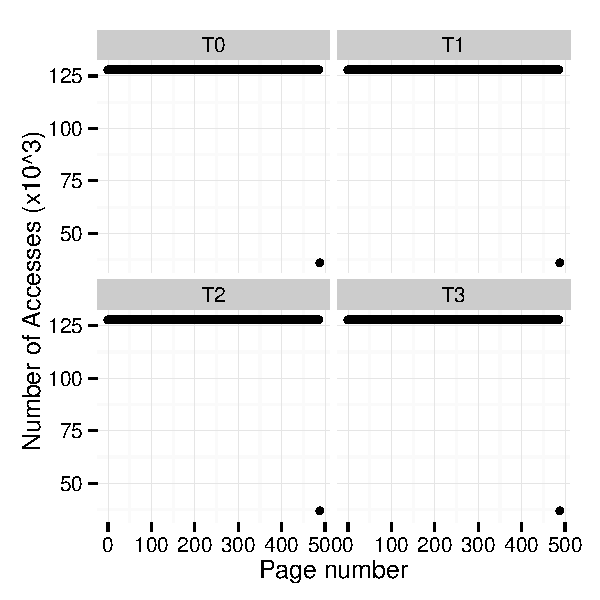
\includegraphics[width=.45\linewidth] {mat_C_modulo}
%         \label{fig:matrix-C-naive}
%     }
%     \subfigure[Structure B (block version).]{
%         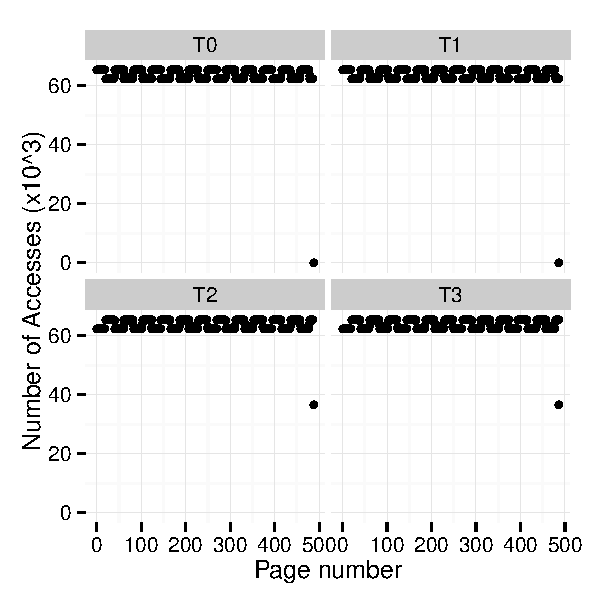
\includegraphics[width=.45\linewidth] {mat_B_bloc}
%         \label{fig:matrix-B-bloc}
%     }
%     \subfigure[Structure C (block version).]{
%         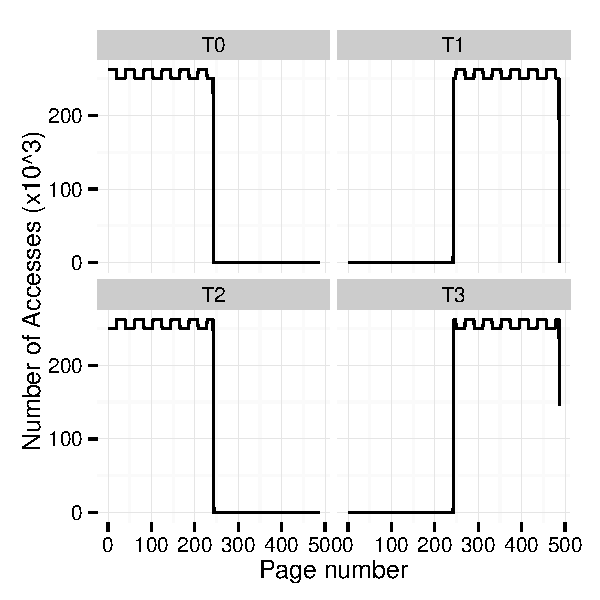
\includegraphics[width=.45\linewidth] {mat_C_bloc}
%         \label{fig:matrix-C-bloc}
%     }
%     \caption{Per-thread access distribution on data structures B and C for the
%     matrix multiplication.}
%     \label{fig:matrix-analysis}
% \end{figure}
% % The figures presented in this sections are part of the \TABARNAC visualization.
% The analysis of the matrix multiplication is shown in Figure~\ref{fig:matrix-analysis}.
% Each plot shows the number of memory accesses for a particular data structure
% per page and per thread. Only structures \texttt{B} and \texttt{C} are
% presented, since \texttt{A} has a very similar access
% pattern as \texttt{C} for both implementations.
% For the naive matrix multiplication, all pages of both structures are used by every
% thread, as we can see in
% Figures~\ref{fig:matrix-B-naive}~and~\ref{fig:matrix-C-naive}. Therefore, when we execute this code on a NUMA machine, wherever we
% map the page, all the nodes but one will trigger remote memory accesses. There
% are several ways to improve this behavior: an easy solution
% is to tell the operating system to interleave pages through the different
% nodes. This will result in a better balance of memory bandwidth between the
% nodes. Another solution is to create local copies of \texttt{A} and
% \texttt{B} on each node as these matrices are only read. Finally, we can modify
% the algorithm to improve the locality, which means using the block algorithm.

% %\begin{figure}[htb]
% %    \centering
% %    \subfigure[Structure B (block version).]{
% %        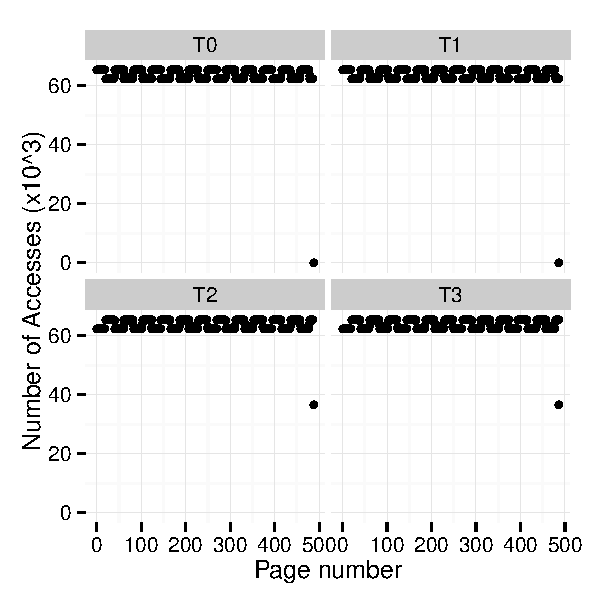
\includegraphics[height=.24\textheight] {mat_B_bloc}
% %        \label{fig:matrix-B-bloc}
% %    }
% %    \subfigure[Structure C (block version).]{
% %        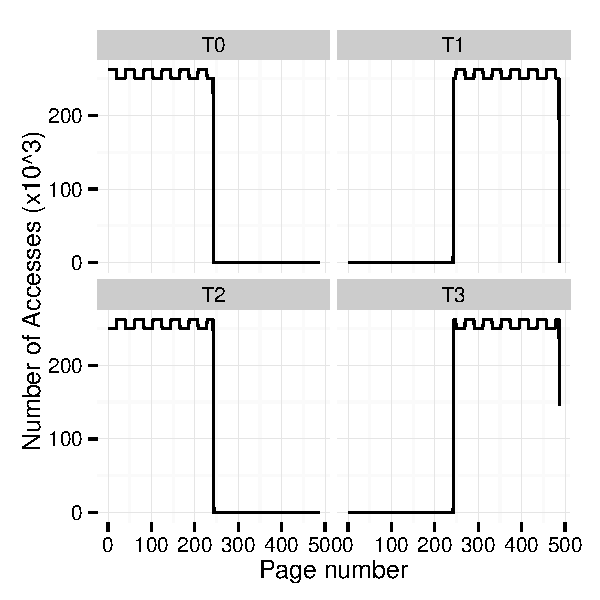
\includegraphics[height=.24\textheight] {mat_C_bloc}
% %        \label{fig:matrix-C-bloc}
% %    }
% %    \caption{By thread access distribution on data structures A and B for the
% %    block matrix multiplication.}
% %    \label{fig:matrix-bloc}
% %\end{figure}

% As we can see in Figures~\ref{fig:matrix-B-bloc}~and~\ref{fig:matrix-C-bloc}, the block algorithm improves the page
% locality compared to the naive implementation. In our algorithm, structures \texttt{B}
% and \texttt{C} are not divided the same way, resulting in two different access patterns. For structure \texttt{B} (Figure~\ref{fig:matrix-B-bloc}), the pages still
% have similar numbers of accesses for all threads. Structures \texttt{C} and
% \texttt{A} (Figure~\ref{fig:matrix-C-bloc}) are split in two parts. The first half
% is shared by threads $T0$ and $T2$ while the two others work on the second
% half. This behavior provides strong page locality and is therefore more
% suitable for NUMA machines. We can easily put each part of \texttt{C} (and
% \texttt{A}) on a NUMA node and map the threads using them to this node, while matrix
% \texttt{B} can be distributed using an interleave policy.

% To evaluate the performance improvements of the proposed modifications, we compare the execution
% time of both versions of the code (naive and block) with the mapping suggested by \TABARNAC to the original Linux kernel (base), and to NUMA Balancing.
% For the naive version, the interleave policy is identical to \TABARNAC and is therefore not shown separately.
% We use bigger matrix for the block version than for the naive one as this
% algorithm is designed to benefit from cache and thus reduce the impact of NUMA
% mapping policy.


% \begin{figure}[htb]
%     \centering
%     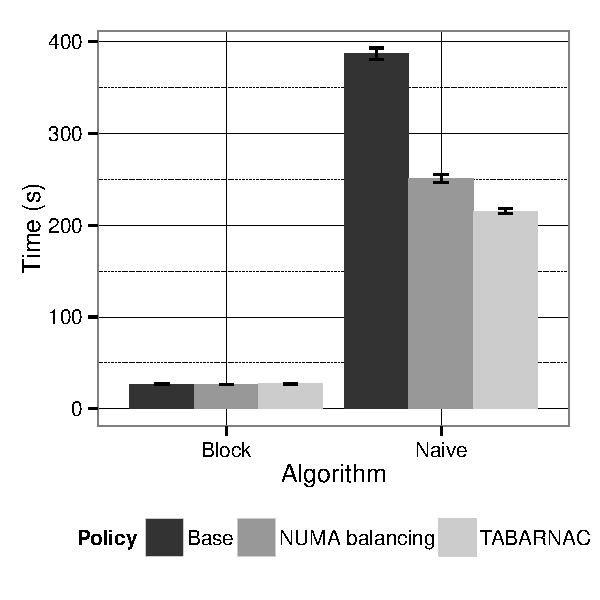
\includegraphics[width=.7\linewidth]{mat_time}
%     \caption{Speedup of the matrix multiplication for size $4096 \times 4096$
%     doubles (naive) and size $8192 \times 8192$ doubles (block).}
%     \label{fig:matrix-res}
% \end{figure}

% Figure~\ref{fig:matrix-res} shows the experimental results of the matrix multiplication. We can see that for
% the naive algorithm, NUMA Balancing is already quite efficient and results in a $40\%$
% speedup. However, using the \TABARNAC policy avoids the runtime overhead and
% allows us to obtain almost $50\%$ of speedup. For the block version, even with
% matrix $4$ times bigger, all policies provide similar execution times, as this
% algorithm is designed to fit in the caches of the system, such that the NUMA
% policy should not influence the results.

% This example shows
% how \TABARNAC can help improving an application by highlighting an inefficient
% memory access behavior. This knowledge can be used two different ways, and always
% results in significant performance improvements. Either the user can modify the code to
% improve the access distribution (in this case going from the naive to the block version),
% or at least \TABARNAC will help choosing the best NUMA page mapping policy.

\subsection{Ondes3D}
\label{sec:exp-ondes3d}

\emph{Ondes3D} is the main numerical kernel of the Ondes3D
application~\cite{Dupros2008}. It simulates the propagation of seismic waves
using a finite-differences numerical method. Ondes3D has a memory usage of
$11.3$Gib with the parameters used for the performance evaluation and $0.7$Gib
for the analysis.

\begin{figure}[htb]
    \centering

    %\subfigure[Original access distribution.]{
    %    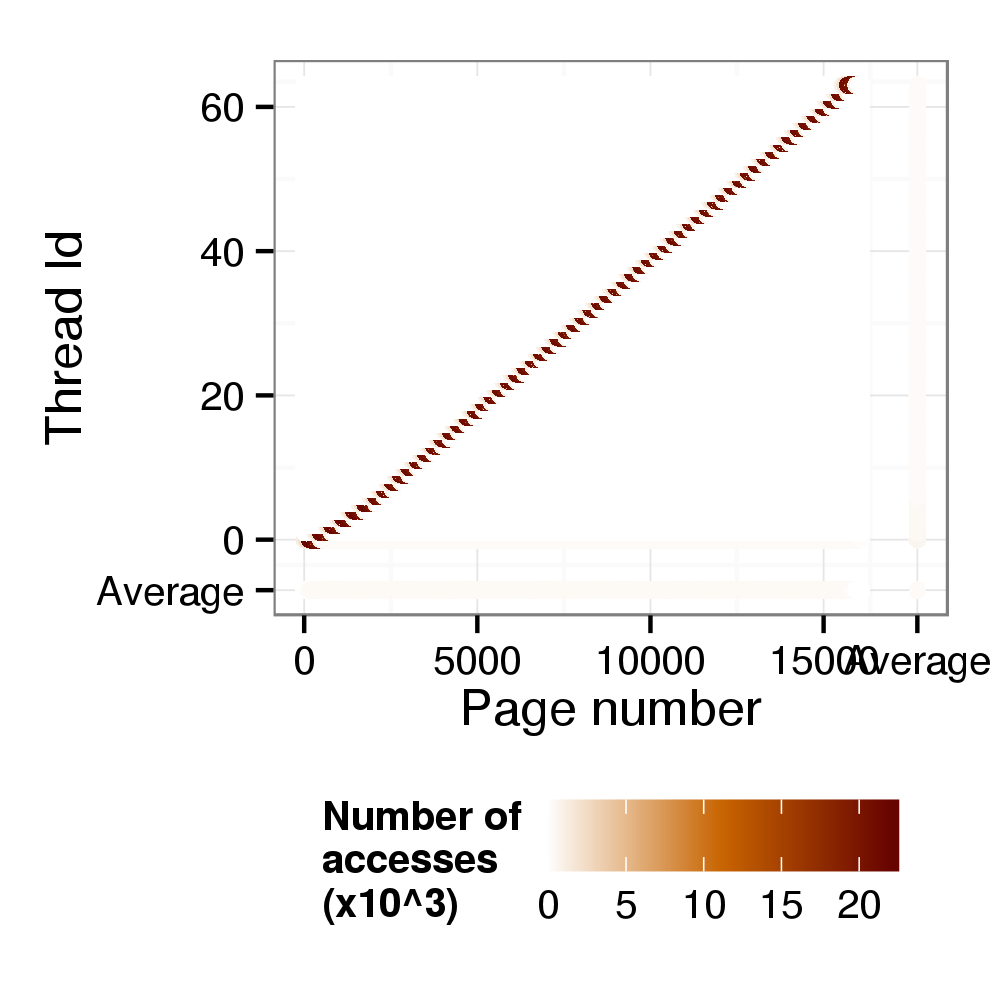
\includegraphics[width=.45\linewidth] {ondes3d_vz0_dist_orig}
    %    \label{fig:ondes3d-behaviour-vz0-orig}
    %}
    %\subfigure[Access distribution after modifications.]{
    %    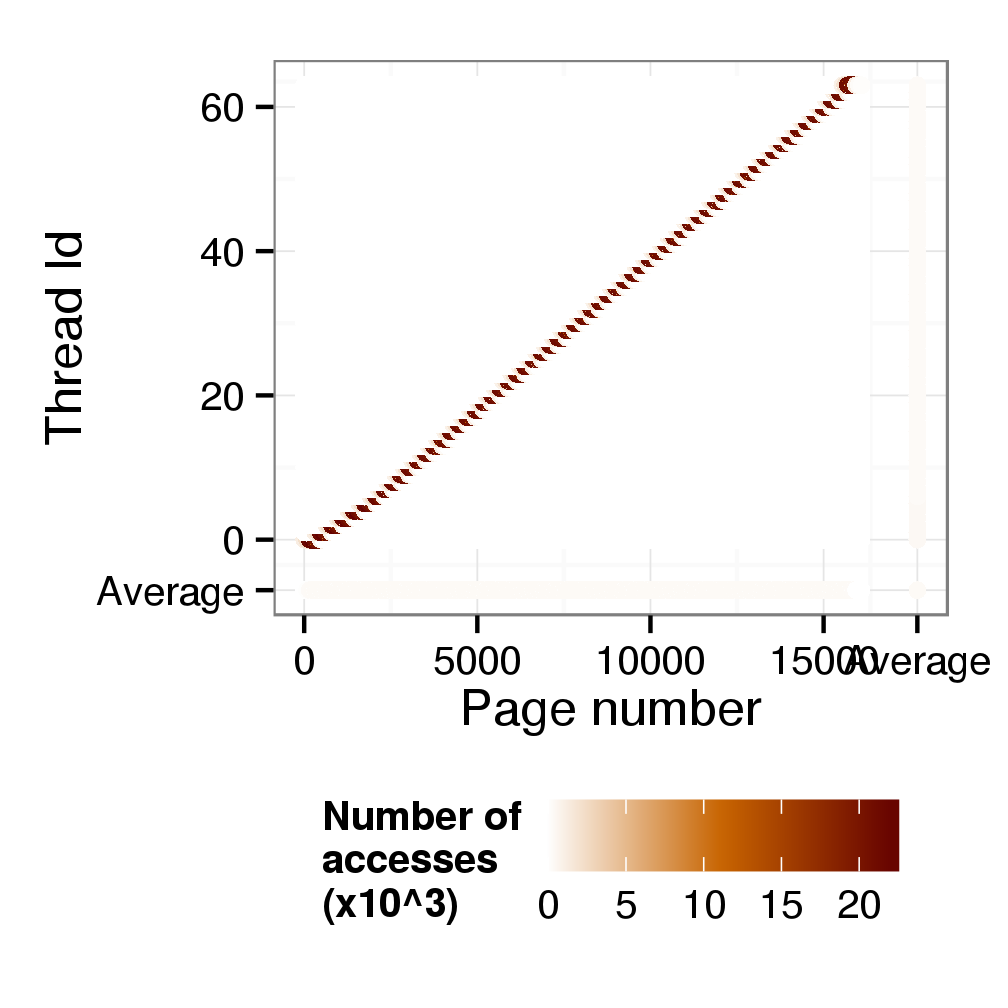
\includegraphics[width=.45\linewidth] {ondes3d_vz0_dist_modif}
    %    \label{fig:ondes3d-behaviour-vz0-modif}
    %}
    \subfigure[Original first-touch.]{
        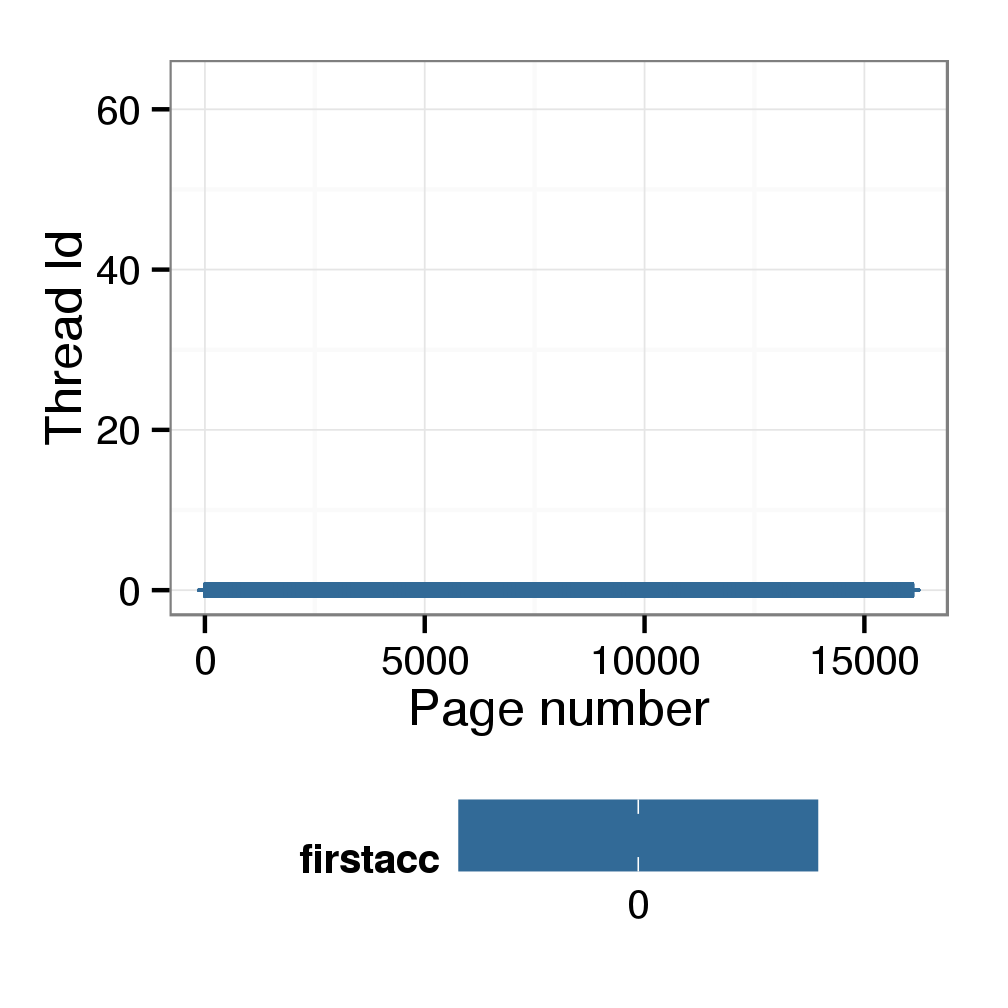
\includegraphics[width=.45\linewidth] {ondes3d_vz0_ft_orig}
        \label{fig:ondes3d-ft-vz0-orig}
    }
    \subfigure[Improved first-touch.]{
        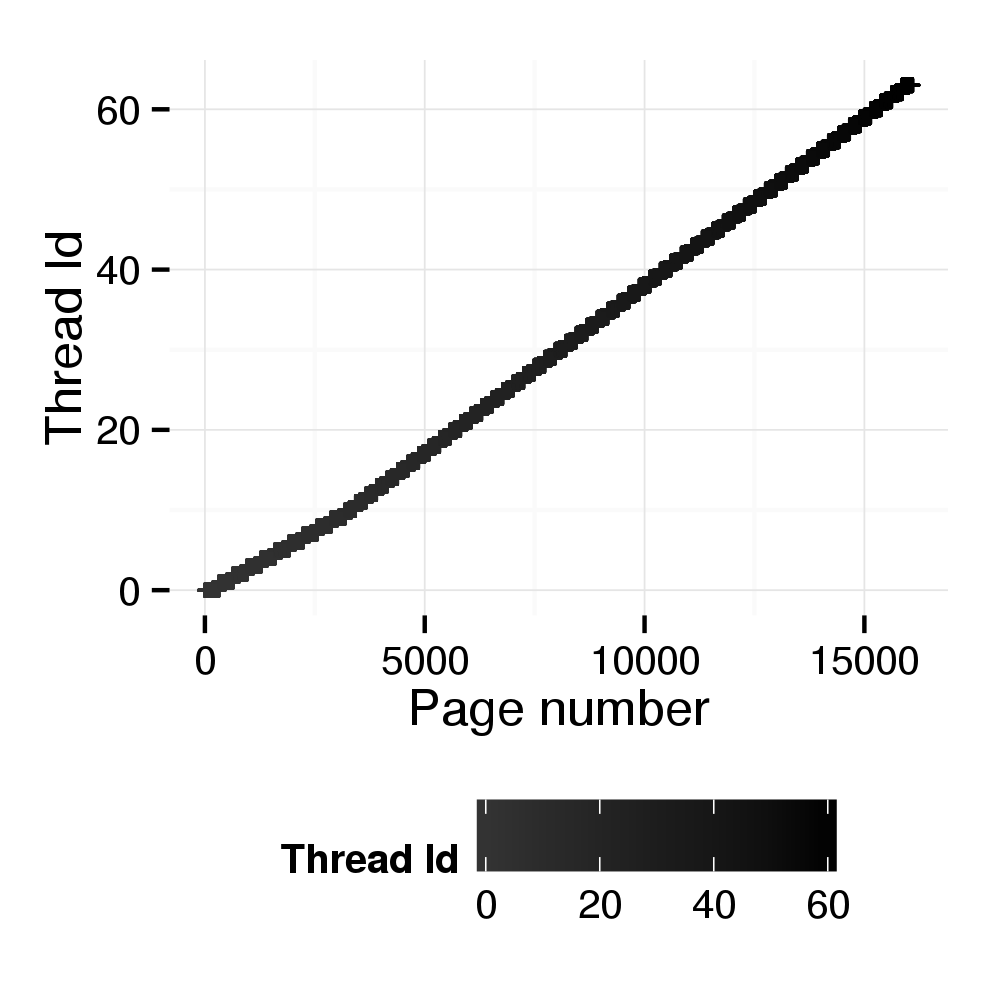
\includegraphics[width=.45\linewidth] {ondes3d_vz0_ft_modif}
        \label{fig:ondes3d-ft-vz0-modif}
    }
    \caption{First-touch for structure
        \texttt{vz0} from \emph{Ondes3D}.} %Original version on the left,
    %modified on the right.}
    \label{fig:ondes3d}
\end{figure}

The analysis of the accesses distribution in \emph{Ondes3D} (not displayed
here) shows that each
structure seems to be well distributed between the threads. %, as we can see for
%structure \texttt{vz0} in Figure~\ref{fig:ondes3d-behaviour-vz0-orig}.
However, for all structures,
thread~$0$ is responsible for all first accesses, as we can see for \texttt{vz0} in
Figure~\ref{fig:ondes3d-ft-vz0-orig}. Due to
this pattern, if we run \emph{Ondes3D} without any improved mapping policy, every page will be
mapped to the NUMA node that executes the thread~$0$, resulting in mostly remote
accesses for the other threads. An easy fix is to perform the initialization
in parallel and to pin each thread on a different core, or to use the
interleave policy.
Such a modification results in the first touch distribution shown in
Figure~\ref{fig:ondes3d-ft-vz0-modif}, which is now distributed among all the threads.

\begin{figure}[htb]
    \centering
    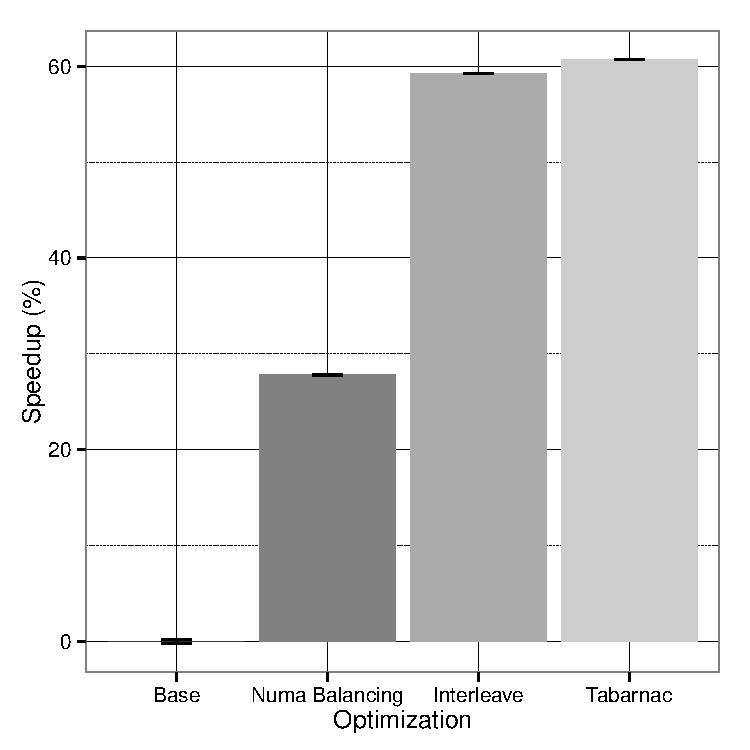
\includegraphics[scale=.55]{ondes3d_exectime}
    \caption{Speedup for \emph{Ondes3D} compared to the baseline.}
    \label{fig:ondes-res}
\end{figure}

We compare the performance of the modified version (\emph{First Touch}) to the
original (\emph{Base})
version, running on the normal OS, with \emph{NUMA Balancing} activated and with an
\emph{Interleave} policy. Figure~\ref{fig:ondes-res} present the results of this
evaluation. We can see that all methods improve the execution time compared to the OS, but
NUMA Balancing provides less than $30\%$ speedup, while the static mappings
(Interleave and the modified code) increase performance by $60\%$.
%This is due to the training time described in Section~\ref{sec:soa-mapping}.
Indeed,
with \emph{NUMA Balancing}, all pages are initially mapped by the OS to the NUMA node
of thread~$0$, and
are only moved later on, after many remote accesses have already occurred,
losing some optimization opportunities. This is a case where static mapping can be substantially better than automated
tools. The \emph{Interleave} policy provides a similar speedup as
\emph{First Touch} since it distributes the pages over the NUMA nodes at the beginning of
the execution, but our tool shows clearly the cause of the performances issue.
% Nevertheless, the interleave version only maps the data no the
% threads, therefore the performances might drop if the OS does not map them
% ``correctly'' while the modified version proposes a thread mapping that ensures better
% data locality.


\subsection{The IS Benchmark}
\label{sec:exp-is}

%\tod{i suggest removing the next 2 phrases:}
We executed \TABARNAC on the benchmarks %written in \texttt{C}
from the OpenMP
implementation of the NAS Parallel Benchmark suite~(NPB)~\cite{Jin1999}.
%\tod{there are just 2...}
% David: Actually we tried also some fortran NPB but I didn't insist on
% getting the good structure names as the access patterns were ``good''
Most
of them have either a well balanced accesses pattern between the threads or a
totally random accesses distribution. For all of them, the first touch fits exactly
the access distribution. However, the analysis of \emph{IS} caught our attention.
\emph{IS} sorts a set of integer numbers using a parallel bucket sort
algorithm.
According to the NAS
website\footnote{\url{http://www.nas.nasa.gov/publications/npb.html}}, \emph{IS} has a
random memory access pattern, while we observed a very specific pattern. In this
section we explain this pattern and how we used it to improve the performance of \emph{IS}.

\begin{figure*}[!htb]
    \centering

    \subfigure[\texttt{key\_array} (original).]{
        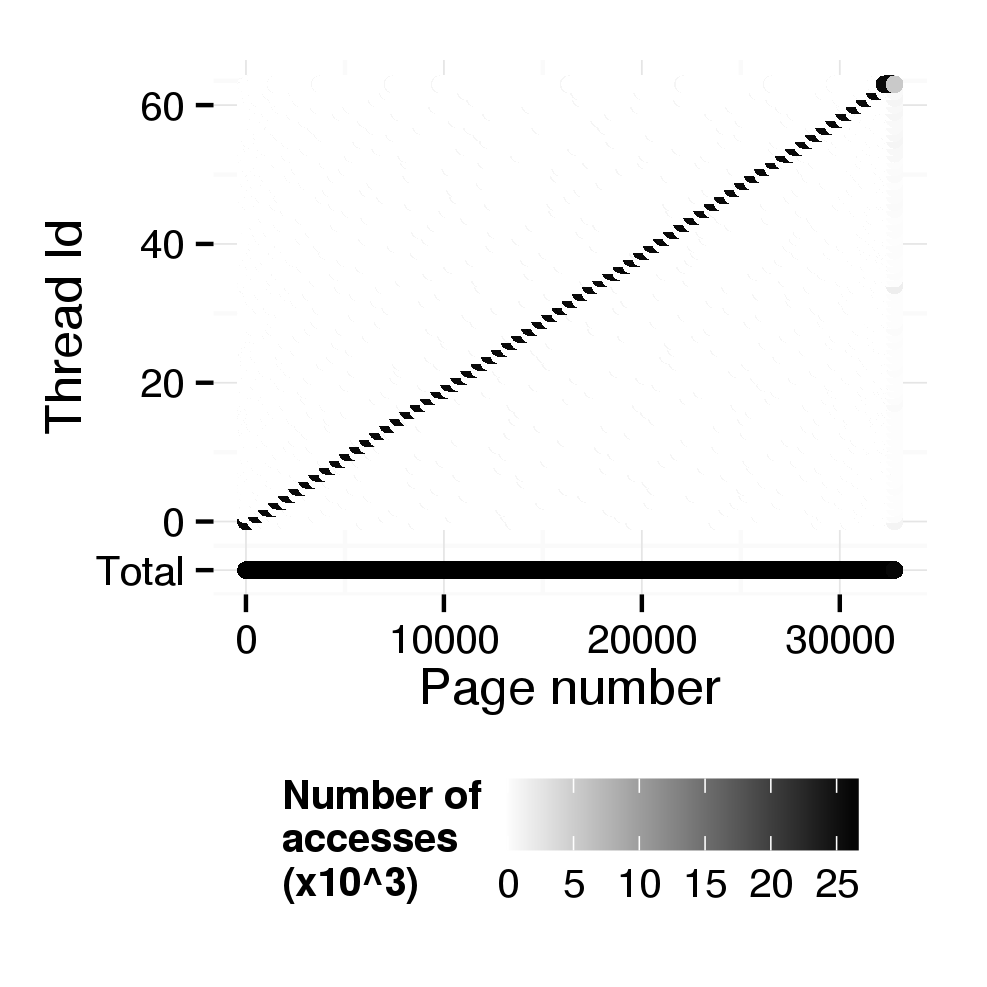
\includegraphics[width=.28\linewidth]  {is_b_kba_orig}
        \label{fig:is-behaviour-orig-kba}
    }
    \subfigure[\texttt{key\_buff2} (original).]{
        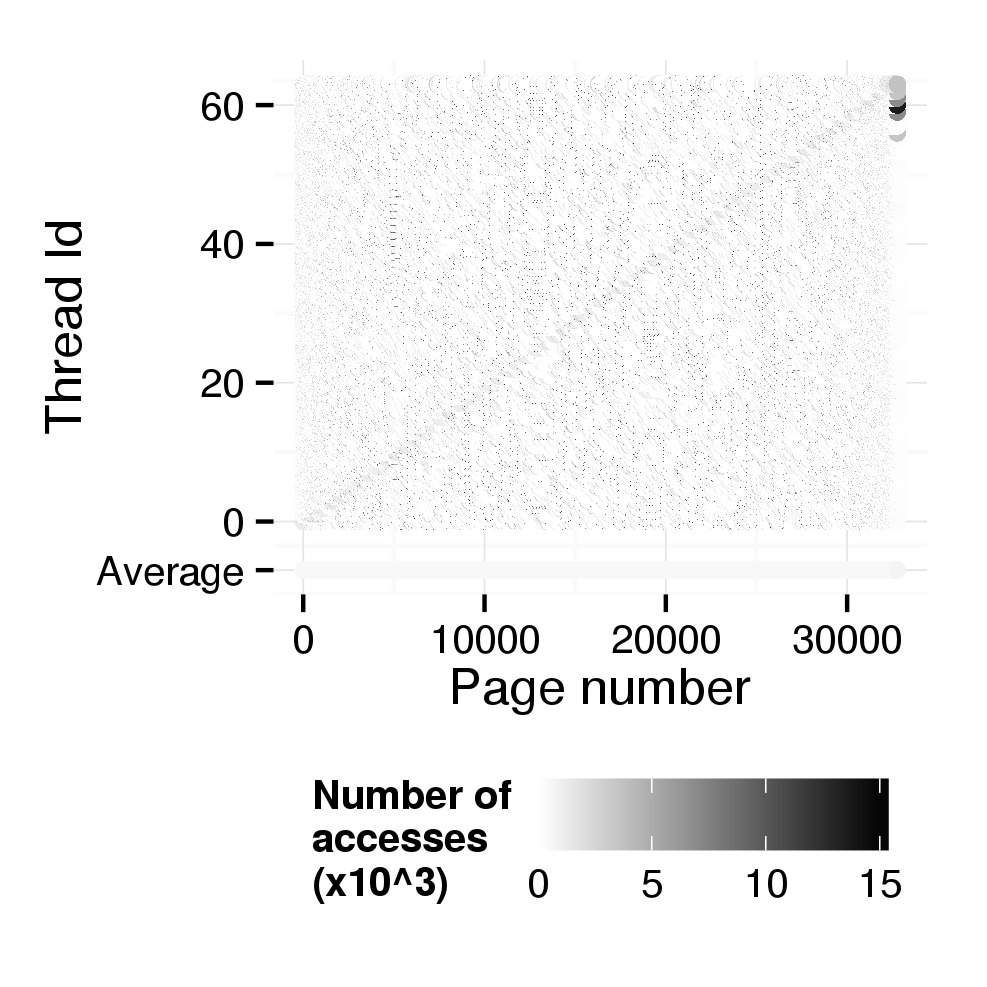
\includegraphics[width=.28\linewidth]  {is_b_kb2_orig}
        \label{fig:is-behaviour-orig-kb2}
    }
    \subfigure[\texttt{key\_buff1} (original).]{
        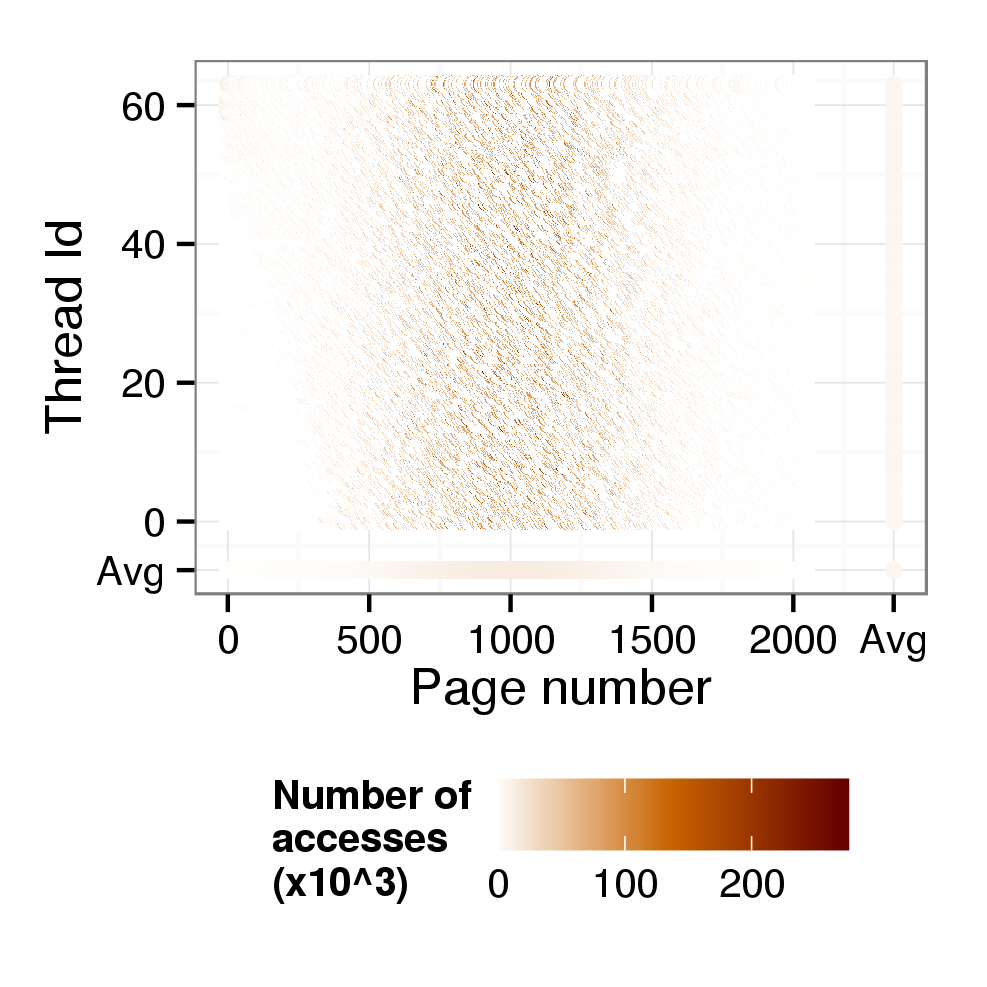
\includegraphics[width=.28\linewidth]  {is_b_kb1_orig}
        \label{fig:is-behaviour-orig-kb1}
    }
    \subfigure[\texttt{key\_array} (modified).]{
        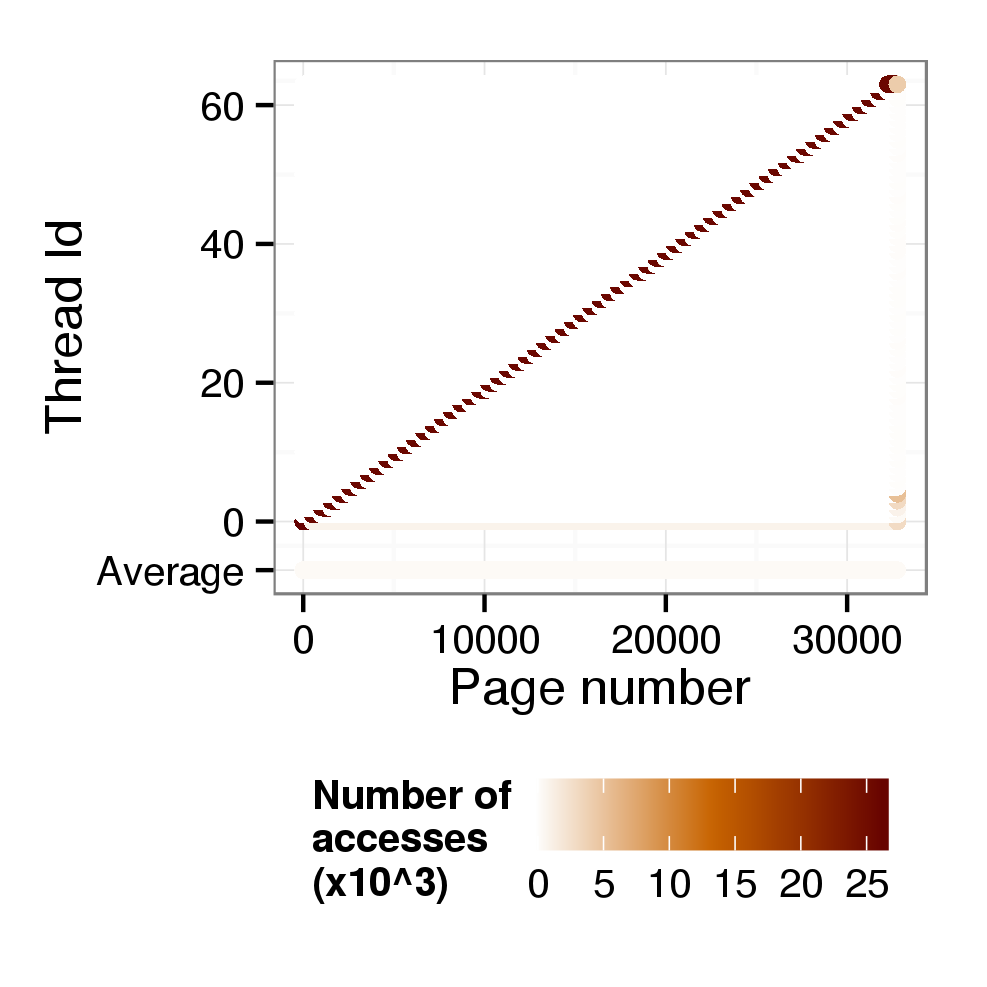
\includegraphics[width=.28\linewidth] {is_b_kba_modif}
        \label{fig:is-behaviour-modif-kba}
    }
    \subfigure[\texttt{key\_buff2} (modified).]{
        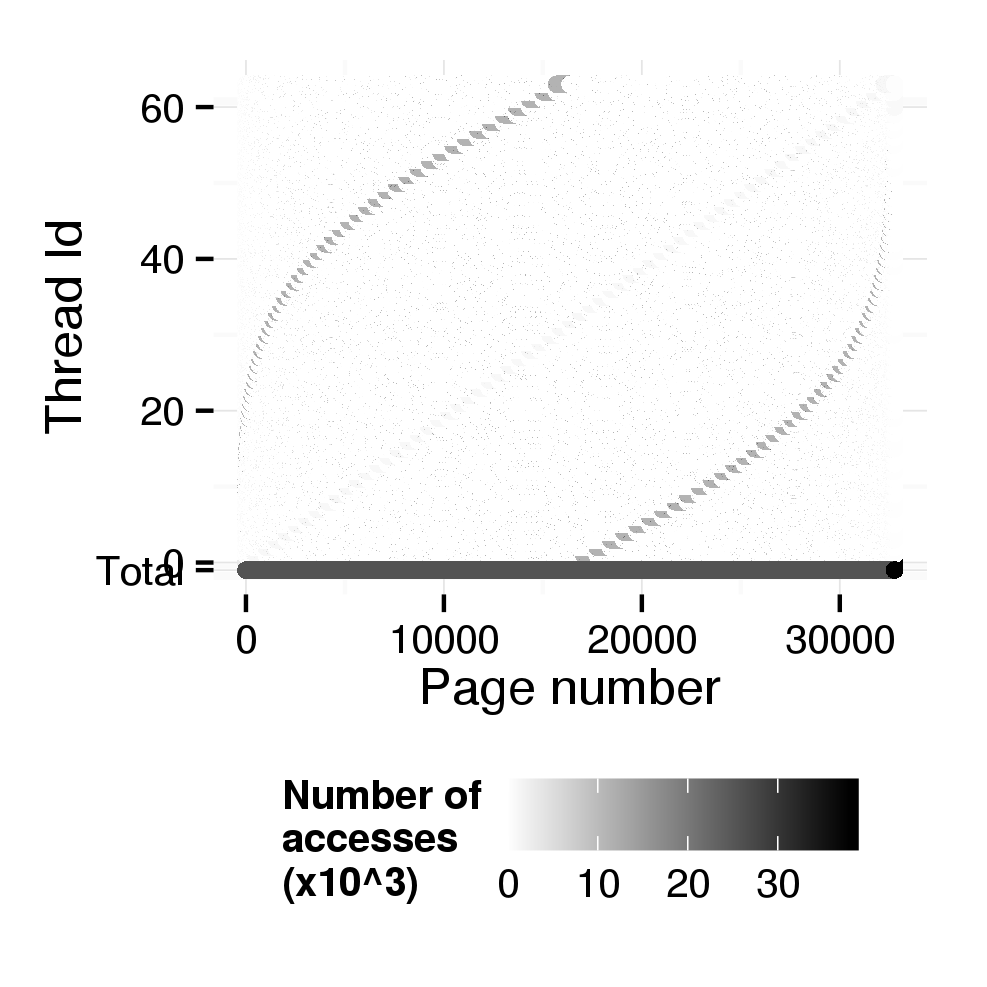
\includegraphics[width=.28\linewidth] {is_b_kb2_modif}
        \label{fig:is-behaviour-modif-kb2}
    }
    \subfigure[\texttt{key\_buff1} (modified).]{
        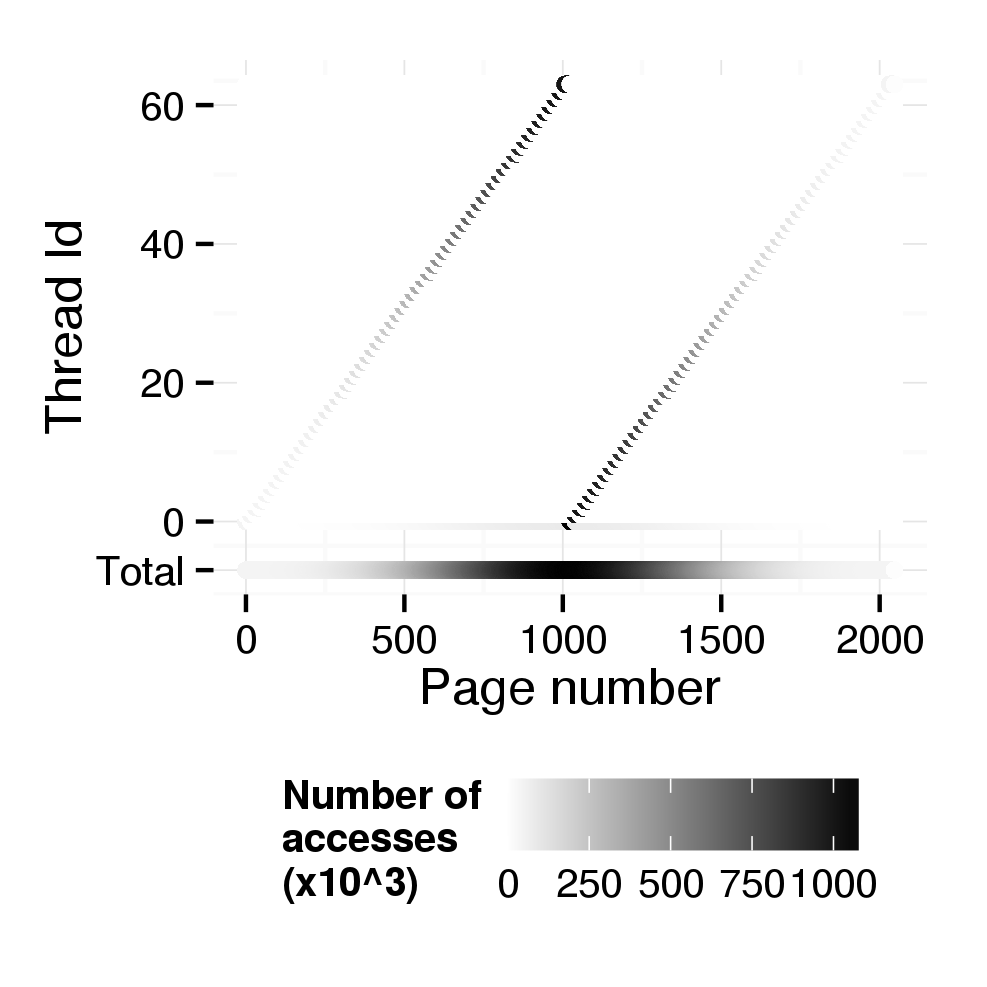
\includegraphics[width=.28\linewidth] {is_b_kb1_modif}
        \label{fig:is-behaviour-modif-kb1}
    }

    \caption{Memory access distribution for the main structures of
        \emph{IS}. Original behavior on the top, modified on
    the bottom.}
    \label{fig:is-behaviour}

\end{figure*}



\emph{IS} was executed with input class \emph{D} for the performance
evaluation, resulting in a memory usage of $33.5$Gib, and class \emph{B} for
the analysis, with a memory usage of $0.25Gib$.

The top of Figure~\ref{fig:is-behaviour} shows the original access distributions for the
three main structures of \emph{IS}. We can see that
each structure has a different access pattern: \texttt{key\_array}'s
(Figure~\ref{fig:is-behaviour-orig-kba}) access distribution shows that each
thread works on a different part of the structure, which permits automated
tools perform an efficient data/thread mapping on it. On the other hand, \texttt{key\_buff2}
(Figure~\ref{fig:is-behaviour-orig-kb2}) is completely shared by all threads.
\texttt{key\_buff1}'s access distribution (Figure~\ref{fig:is-behaviour-orig-kb1})
is the most interesting one. We can see that almost all accesses occur
in pages in the middle of the structure (from page $500$ to $1500$), and those pages
are shared by all threads. This means that the number of access per page  for
each thread follows a Gaussian distribution centered in the middle of the
structure.

%\lstinputlisting[caption=\emph{IS} code responsible for the
%Gaussian distribution of memory accesses to the \texttt{key\_buff1} structure., label=lst:is, float=htb]{code/is.c}

We can identify the source of this pattern in the \emph{IS} source code. Indeed, all the accesses to \texttt{key\_buff1} are linear,
except in one OpenMP parallel loop where they depend on the value of
%except the ones shown in Listing~\ref{lst:is}\footnote{
%    The code has been slightly modified to make it more readable. In the
%    original version, the arrays \texttt{key\_buff1} (resp. \texttt{key\_buff2})
%    are accessed via a generic pointer called \texttt{key\_buff\_ptr} (resp.
%    \texttt{key\_buff\_ptr2}).
%}, line \ref{lst:is-gaus-end}, which depend on the values of
\texttt{key\_buff2}.

As we noticed in Figure~\ref{fig:is-behaviour-orig-kb1} that the values of \texttt{key\_buff2}
follow a Gaussian distribution, we can design a distribution of the threads that
provides both a good load balancing and locality of data.
By default, OpenMP threads are scheduled dynamically to avoid unbalanced
distribution of work, but the developers also propose a cyclic distribution
of the threads over the loop.
For our distribution, we split
the loop into two equal parts and distribute each part among the threads in a round-robin way.
This modification can be done by simply changing one line of code, the
\texttt{\#pragma omp} before the parallel loop.
%This can be done by modifying the OpenMP pragma (line~\ref{lst:is-sched} in the original code), as shown
%in Listing~\ref{lst:is-modif}.

%\begin{lstlisting}[float=!h,caption=Optimization for \emph{IS}., label=lst:is-modif]
%#pragma omp for schedule(static,NUM_BUCKETS/(2*omp_get_num_threads()))
%\end{lstlisting}


With this code modification, we obtain the access distribution shown in
the bottom of Figure~\ref{fig:is-behaviour}. We can see that now each thread
accesses a different part of \texttt{key\_buff1}. Furthermore, if most of the
accesses still occur in the middle of the structure, the average number of
access across the structure is the same for all threads, which means that our
distribution preserves the good load balancing. Our modification has also
changed \texttt{key\_buff2}'s accesses distribution. We can see that each
thread uses mostly one part of the array and again the load balance is
preserved.

The main point of our code modification is to improve the affinity between
thread and memory, therefore we need to pin each thread on a core to keep them
close to the data they access. %To perform the thread mapping, we use the \texttt{GOMP\_CPU\_AFFINITY} environment variable.
\TABARNAC also shows us that the first touch is always done by the thread actually using
the data for IS, therefore we do not need to explicitly map the data to the NUMA nodes.

We compare the execution time of \emph{IS} (class \emph{D}) for the three scheduling
methods, \emph{Dynamic}, \emph{Cyclic} with a step of $1$ and \emph{Cyclic-Split}:
cyclic with the proposed distribution. For the two first methods, we compare the
execution time on the base operating system, the interleave policy and with
NUMA balancing enabled. As we map threads manually, interleave and NUMA
Balancing are not relevant with our modifications and are therefore not evaluated.

\begin{figure}[htb]
    \centering
    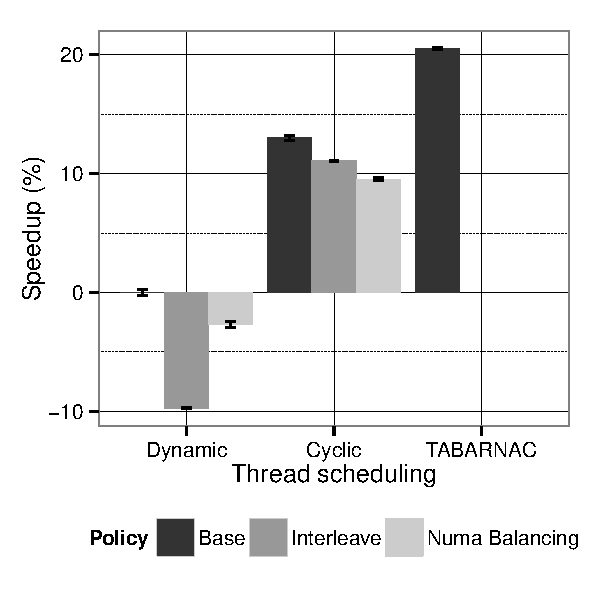
\includegraphics[scale=.65]{is_exectime}
    \caption{Speedup for \emph{IS} (class D) compared to the baseline.}
\label{fig:is-res}
\end{figure}

Figure~\ref{fig:is-res} shows the speedup of \emph{IS} compared to
the default version (\emph{Dynamic}) for each scheduling method and for each
optimization technique. The first thing to notice is that with the default
\emph{Dynamic} scheduling, both Interleave and NUMA Balancing slow
the application down, by up to $10\%$.
This shows that simple optimization policies can actually reduce performance
for NUMA-unaware code.
The \emph{Cyclic} scheduling, proposed in the original code, already provides up to $13\%$ of
speedup. We can see that both interleave and NUMA Balancing are not suitable
for this scheduling, since they reduce the performance gains.
The \emph{Cyclic-Split} version provides more than $20\%$ of speedup with a very small code
modification.
This example shows how analyzing an application's memory behavior can lead to
significant execution time improvement on an already optimized application where automatic techniques can actually slow
the application down.




\subsection{Overhead Analysis}
\label{sec:expe-overhead}

Our last experiment aims at evaluating the instrumentation cost. To do so, we
executed all of the NAS Parallel Benchmarks in class \emph{B} with $64$
threads on both machines and compared the original execution time to the execution time with instrumentation enabled.

\begin{figure}[!htb]
    \centering
    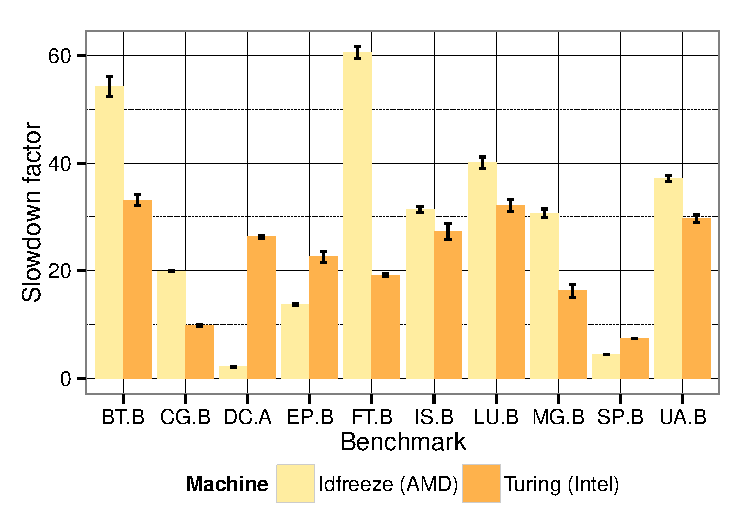
\includegraphics[scale=.65]{tool-ovh.pdf}
    \caption{\TABARNAC's instrumentation overhead.}
    \label{fig:ovh}
\end{figure}

%\begin{table}
%    \centering
%    \begin{tabular}{lrrrrr}
%        \toprule
%        %\multirow{2}{*}{Machine}
%         & \multicolumn{5}{c}{Benchmark (CLASS)} \\
%        \cmidrule(lr){2-6}
%            &\texttt{DC} (A) &\texttt{SP} (B)&\texttt{CG} (B)&\texttt{MG} (B)&\texttt{FT} (B) \\
%        \cmidrule(lr){2-6}
%        \texttt{Turing} &$26.26$ & $7.37$ &$9.75 $ &$16.23$ &$19.17$ \\
%        \texttt{Idfreeze} &$4.30$  & $4.07$  &  $19.92$ &   $30.66$ &    $60.54$ \\
%        \midrule
%        \midrule
%                &\texttt{EP} (B)&\texttt{IS} (B)&\texttt{UA} (B)&\texttt{LU} (B)&\texttt{BT} (B)\\
%        \cmidrule(lr){2-6}
%        \texttt{Turing} &$22.56$ &$27.28$ &$29.65$ &$32.13$ &$33.13$ \\
%        \texttt{Idfreeze} & $13.64$ &$31.32$ & $37.17$ &  $40.05$ &   $54.22$ \\
%        \bottomrule
%    \end{tabular}
%    \caption{Slowdown factor of \TABARNAC instrumentation for the 10 NAS Parallel
%        Benchmarks on both machines.}
%    \label{tab:ovh}
%\end{table}

As we can see in Figure~\ref{fig:ovh}, on the Intel machine,
the instrumentation slows the execution down by a factor from $10$ to $30$.
On the AMD machine, the overhead is almost always higher, and for
pathological cases, is two to three times slower than on
the Intel machine.
%On most benchmarks, the instrumentation is $10$ to $50\%$ slower on
%AMD than on Intel processor. For the pathological cases (\texttt{FT} and
%\texttt{BT}) the instrumentation can be two or three time slower on AMD.
Although this overhead is not negligible, we have to consider the fact that often we can instrument
smaller versions of the applications, as we focus on the general behavior.
Moreover our method is more precise than sampling and
thus one run is often enough. Finally, as our
analysis is designed to be used during development phase and at runtime in an
automated tool, this overhead is acceptable.

\subsection{Summary}

Our experiments have highlighted the fact that although automated tools such
as NUMA Balancing can be efficient, in some cases they result in
performance losses. Moreover, although simple static mapping policies
can result in substantial improvements, the best policy depends on the memory
accesses behavior of the parallel application. Therefore, it is necessary to understand its memory behavior to
select the most appropriate mapping policy.

Our tools and methodology enables developers and users to achieve performance improvements in two ways. First, by
providing a deep understanding of the memory access behavior, it enables the user to
find the best mapping policy. Second, this knowledge can be used to
identify and fix inefficient memory behavior. Our experiments showed that both
situations result in significant performance gains.
